\documentclass{article}
\usepackage{graphicx}
\usepackage{hyperref}
\usepackage{caption}
\usepackage{subcaption}
\usepackage{mathtools}
\usepackage[dutch]{babel}

\begin{document}

\begin{center}
	\huge{Wiskunde in Kunst}\\
	\LARGE{Opdracht }8 \\
	
	\vspace{2cm}
	
	\Large{De Fibonacci reeks}\\
	
	\vfill
	
	\begin{figure}[Hh]
		\centering
		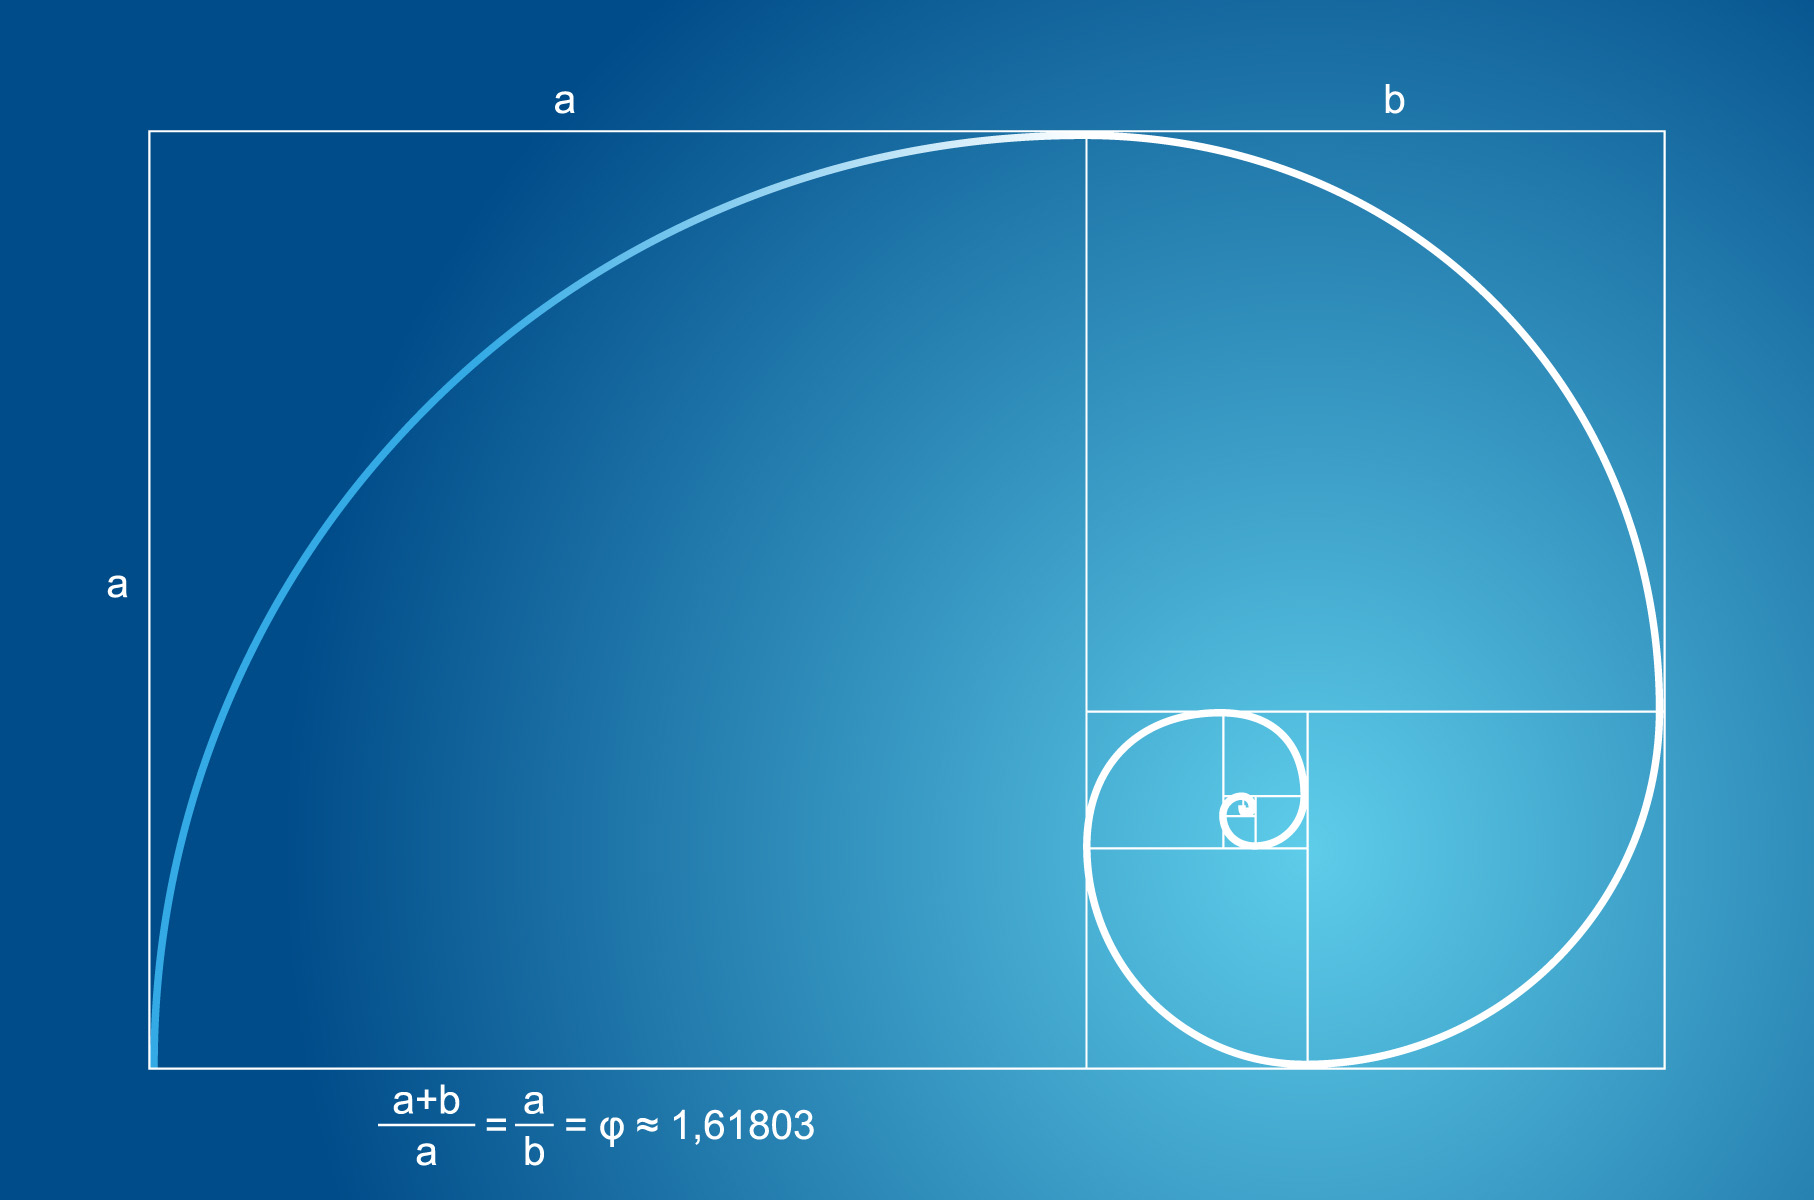
\includegraphics[width=\textwidth]{golden-ratio.jpg}
	\end{figure}
	
	\vfill
	\Large{Marcelo Dias Avelino} \hfill \large{0840416}
\end{center}

\thispagestyle{empty} % Remove page numbering

\pagebreak

\setcounter{page}{1} % Start counting pages here

\section{De wiskundige}

De Fibonnaci reeks is een reeks van getallen die genoemd zijn naar de italianse wiskundige Leonardo Pisano Bigollo. Fibonnaci was geboren op 1170, zon van een rijke handelaar genaamd Guglielmo Bonacci. Zijn vader was een simpele dwaas en was bijgenaamd Bonaccio, wat `dwaas' betekende in de idioom destijds. Hieruit is ook de naam Fibonacci onstaan, wat `zoon van een dwaas' betekent. Zijn vader was consul voor Pisa en eigenaar van een handelspost in B\'eja\"ia, een havenstad oost van Algiers, de hoofdstad van Algerije. Als kleine jonge reisde Fibonnaci heel vaak met zijn vader naar Algerije om hem te helpen en tijdens zijn verblijf daar heeft hij de Hindu-Arabische getallen stelsel geleerd. Hij erkende dat deze getallen stelsel veel effienc\"ienter was om mee te rekenen dat de romeinse stelsel dat destijds nog gebruikt werd overal in Europa en besloot om door het hele Mediterraanse wereld te reizen om onder de arabische wiskundige meesters te leren.

In 1202, toen Fibonnaci 32 was, heeft hij alles wat hij heeft geleerd opgeschreven in een boek genaamd \textit{Liber Abaci} (Boek van Berekeningen). Hierdoor was de Hindu-Arabische getallen stelsel bekend geworden in Europa en vanwege de verbeteringen in effici\"entie in boekhouding, het vertallen van gewichten en metingen, en andere toepassingen is het uiteindelijk compleet overgenomen als standard stelsel. Dit boek bepleitte het gebruik van de cijfers 0 t/m 9 en het gebruik van de positiestelsel. 

De positiestelsel is de systeem dat cijfers hun waarde toekent gebaseerd op hun positie binnen een getal. Dit door elke cijfer te vermenigvuldigen met het aantal symbolen gebruikt in het getallenstelsel, in dit geval 10 symbolen (0 - 9), tot de macht te verheffen van de positie van het getal (beginnend op 0), en alle waardes uiteindelijk bij elkaar op te tellen. Bijv. bij het getal \textit{153}, de positie van het getal 3 bepaalt dat zijn waarde \(3 \times 10^0 = 3\) is, het getal 5 wordt \(5 \times 10^1 = 50\) en het getal 1 wordt \(1 \times 10^2 = 100\). Alles bij elkaar opgeteld komt weer op het getal \(3 + 50 + 100 = 153\) uit.

Uit alle wiskundig kennis opgenomen in dat boek, is de Fibonacci reeks het bekendste geworden.

\begin{figure}[Hh]
	\centering
	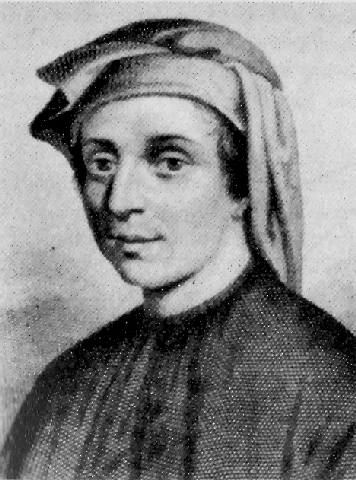
\includegraphics[width=0.3\textwidth]{Fibonacci.jpg}
	\caption{Portret van Fibonnaci door onbekende auteur.}
\end{figure}

\pagebreak

\section{De reeks}

Deze reeks is niet oorspronkelijk bedacht door Fibonacci zelf en wordt al genoemd in het boek \textit{Chhandah-sh\=astra} (Kunst van de Versmaat), geschreven door de Indiase schrijver Pingala tussen 200 - 450 voor Christus. De reeks was hier \textit{maatraameru} (Berg van de cadens) genoemd. Het is mogelijk dat Fibonacci tijdens zijn verblijf bij de arabische meesters deze reeks is tegengekomen.

De reeks volgt de definitie `\(F_n = F_{n-1} + F_{n-2}\)' en begint meestal bij 1. Het pakt de twee vorige getallen en telt ze bij elkaar op om de volgende getal te berekenen, dus \(1 + 1 = 2\), \(1 + 2 = 3\), \(2 + 3 = 5\), en zo voort. Dit betekent dat volgens deze regels de rij als volgt uit ziet: 

\(1,\;1,\;2,\;3,\;5,\;8,\;13,\;21,\;34,\;55,\;89,\;144,\; \ldots\;, \infty\)

Fibonacci heeft de reeks in \textit{Liber Abaci} opgenomen om een probleem over konijnenpopulatie te bestuderen, daarom is de Fibonacci reeks ook bekend als de konijnenreeks. Door de volgende regels te volgen, kon hij het aantal konijnen berekenen na elke maand:

\begin{itemize}
\item{In het begin is er geen paar en in de eerst maand is er \'e\'en paar konijnen.}
\item{Een konijnenpaar wordt volwassen na de tweede maand.}
\item{Elke volwassen paar krijgt na \'e\'en maand een paar nakomelingen.}
\item{De konijnen overlijden niet.}
\end{itemize}

De aantal konijnen na elke maand kwam hierdoor precies uit op de Fibonacci reeks. Dit is een voorbeeld van meerdere waarbij de Fibonacci reeks voorkomt in de natuur. De reeks heeft een sterke verband met de \textit{gulden snede}, een getallen constante dat heel vaak voorkomt in de natuur, zoals bijvoorbeeld bij bomenbladeren dat met een bepaalde afstand van elkaar groeien op een tak. De gulden snede komt neer op \(\varphi \approx 1{,}618\) en als elke getal uit de reeks door het voorgaande getal gedeelde wordt dan zal een benadering van de gulden snede uitkomen. Bijv. \(5/3 \approx 1.67\), \(8/5 \approx 1.6\) en \(89/55 \approx 1.618\).

\end{document}
